\chapter{Аналитический раздел}
\label{cha:analysis}

\section{Задача поиска шаблонов проектирования}

Шаблон проектирования системным образом называет, определяет причины и
разъясняет в общем виде проблему повторимости некоторой конструкции в
объектно-ориентированных системах.
Описывает не только задачу, но и решение, когда его применить, и к каким
последствиям это приведет.
Также предоставляет примеры и советы по реализации.
Решение --- это общая структура объектов и классов, которая решает задачу.
Оно варьируется и его реализация зависит от контекста задачи~\cite{DesignPatterns}.

Из этого определения можно выделить следующие особенности шаблонов проектирования,
которые необходимо учесть при описании структуры:
\begin{enumerate}
\item описание конструкции в общем виде --- означает, что нужно иметь механизм,
который позволит уйти от конкретных типов данных, различного рода идентификаторов;
\item повторимость конструкции --- описание шаблона должно определять все
возможные конструкции в системе, подпадающие под этот шаблон;
\item описывает решение --- шаблоном может быть часть программы написанная на
любом объектно-ориентированном языке.
\end{enumerate}

Целью для поиска должна быть некоторым образом формализованная
объектно-ориентированная система.
Найти готовый проект такой системы, описанный по определенным стандартам
довольно сложно.
Чтобы убедиться в работоспособности метода можно использовать исходный код
программ.
Структура таких проектов точно будет работоспособной, сложность будет только
в построении модели.

Результатом поиска должно быть множество вариантов соответствий структурных
элементов системы элементам шаблона.
В самом общем виде метод представлен на рисунке~\ref{fig:idef0}.
Подробнее на рисунке~\ref{fig:idef0-general}.

\begin{figure}
\centering
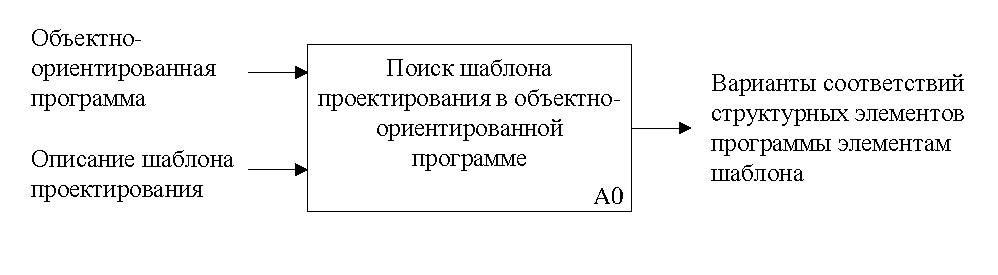
\includegraphics[width=\textwidth]{inc/idef0.pdf}
\caption{Метод поиска шаблонов проектирования в объектно-ориентированных программах}
\label{fig:idef0}
\end{figure}

\begin{figure}
\centering
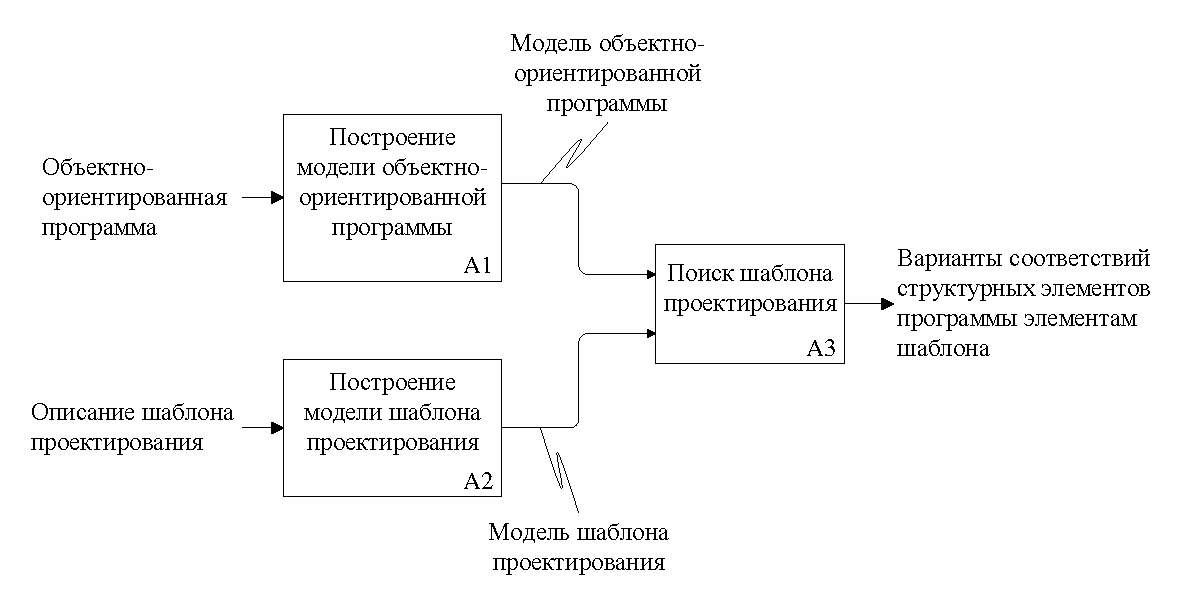
\includegraphics[width=\textwidth]{inc/idef0-general.pdf}
\caption{Метод поиска шаблонов проектирования в объектно-ориентированных программах с использованием моделей программы и шаблона}
\label{fig:idef0-general}
\end{figure}

\section{Анализ существующих методов поиска шаблонов проектирования}

Основным подходом решения поставленной задачи является сведение её к поиску
изоморфного подграфа.
Кратко рассмотрим возможные модификации такого подхода.

\subsection{Анализ метода поиска шаблонов проектирования с использованием меры схожести}

\cite{DesignPatternSimilarityScoring}

\subsection{Анализ метода поиска шаблонов проектирования с использованием поиска по образцу}

\cite{DesignPatternTemplateMatching}

\section{Алгоритмы поска изоморфных подграфов}

Задача поиска изоморфного подграфа является \textbf{NP}-полной.
Точное решение задачи в общем случае занимает экспоненциальное время.
Можно решить задачу за полимиальное время, но с некототорой точность.
Рассмотрим соответствующие алгоритмы.

\subsection{Алгоритмы поиска изоморфного подграфа на основе меры схожести вершин}

\cite{SimilarityGraphVertices}

\subsection{Алгоритмы поиска изоморфного подграфа на основе метода поиска с возратом}

\cite{SubgraphIsomorphism}

\section{Метод поиска шаблонов проектирования в объектно-ориентированных программах на основе поиска изоморфных подграфов}

%\begin{figure}
%\centering
%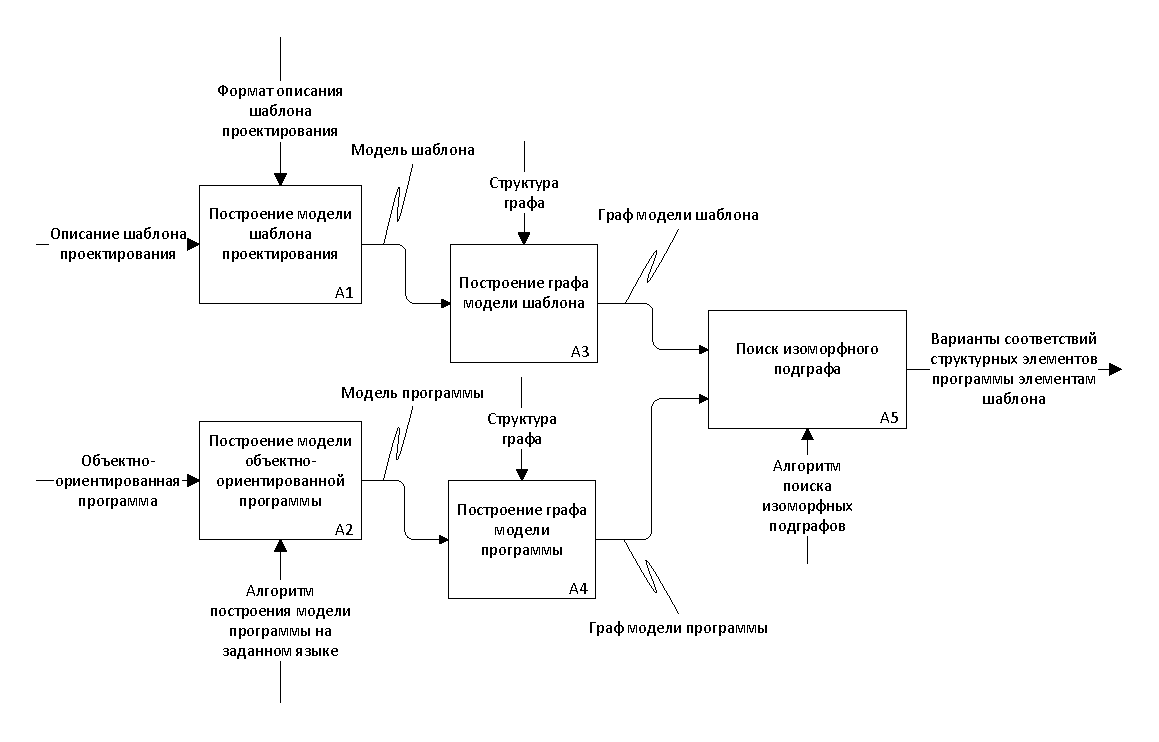
\includegraphics[width=\textwidth]{inc/idef0-specific.pdf}
%\caption{Метод поиска шаблонов проектирования в объектно-ориентированных программах на основе поиска изоморфных подграфов}
%\label{fig:idef0-specific}
%\end{figure}
